\documentclass{beamer}
\mode<presentation>

\usepackage[english]{babel}
\usepackage[utf8x]{inputenc}
\usepackage{amsmath}
\usefonttheme{serif}
\usetheme{Boadilla}
\usepackage{listings}
\lstset{language=R}
\newcommand{\Mod}[1]{\ (\text{mod}\ #1)}
\newcommand\floor[1]{\lfloor#1\rfloor}
\newcommand\ceil[1]{\lceil#1\rceil}
	
\title{Time Series Analysis}
\author{Venkatramani Rajgopal}
\institute[] 
{\	Department of Mathematics\\
		University of Applied Sciences, Mittweida}
	

\date{3 Nov 2016} 
\subject{}
\begin{document}

\begin{frame}
\titlepage
\end{frame}

\begin{frame}{Outline}
\tableofcontents
% You might wish to add the option [pausesections]
\end{frame}		


\section{Introduction}
\begin{frame}{Introduction}
\begin{block}{Time Series}
A collection of random variables indexed according to the order they are obtained in time. 
\end{block}

\pause
\begin{itemize}
\item Takes into account the internal structure of data points, such as \textit{autocorrelation, trend or seasonal variations}
\item Modeling relationships using data collected over time. For eg Stock Price, Index Closings, GDP etc.  
\end{itemize}

\end{frame}
\begin{frame}{Introduction}
	\begin{block}{Motivation}
		In the context of; 
		\begin{itemize}
			\item Statistics, econometrics, quantitative finance and geophysics the primary goal of time series analysis is forecasting.
			\item Signal processing, it is used for signal detection and estimation, 
			\item Data mining, pattern recognition and machine learning time series analysis can be used for clustering and classification. 
		\end{itemize}
		
		
	\end{block}
	
\end{frame}


\begin{frame}{Introduction}
\begin{block}{Methods}
	{\small
Methods for time series analysis may be divided into two classes: frequency-domain methods and time-domain methods.
\pause
\begin{itemize}
\item \textit{Frequency domain:} include spectral analysis and wavelet analysis;
\item \textit{Time domain:} include auto-correlation and cross-correlation analysis.  %\\ In the time domain, correlation and analyses can be made in a filter-like manner using scaled correlation, thereby mitigating the need to operate in the frequency domain.}
\end{itemize}
}
\end{block}


\begin{block}{Models in time domain:}

{\small Three broad model classes of practical importance are the autoregressive (AR) models, the moving average (MA) models. These two classes depend linearly on previous data points. \\
	
Combinations of these ideas produce autoregressive moving average (ARMA) and autoregressive integrated moving average (ARIMA) models. }
\end{block}

\end{frame}

\begin{frame}{Introduction}{Nature of Time series data}	
We will try to handle some \textit{ts} data in R using the inbilt dataset in R (JohnsonJohnson). 
	
	\begin{figure}
		\centering
		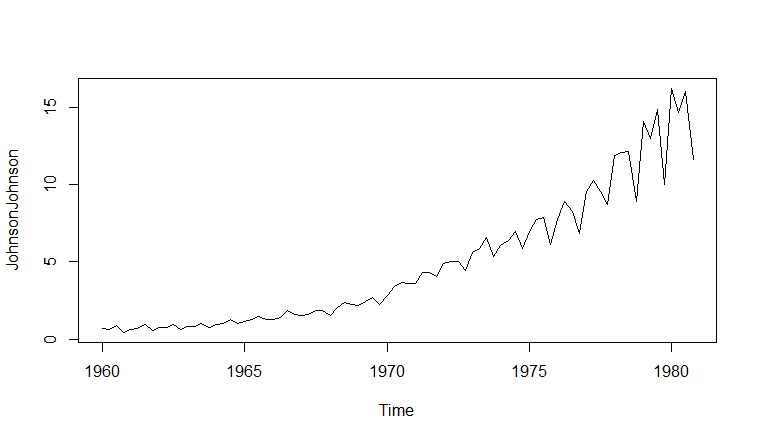
\includegraphics[width=0.7\linewidth]{j&jplot}
	\end{figure}
	{\footnotesize 
		data(JohnsonJohnson)\\
		plot(JohnsonJohnson,type="l")
	}
	
\end{frame}

\section{Classical regression in time series context}
\begin{frame}{Classical regression in time series context}
	Linear regression in the time series context can be done by assuming some output or \textit{time dependent series}, say $ x_t $ for $ t = 1,2 \dots n $ which are being influenced by a collection of possible inputs or independent series, say $ z_{t1}, z_{t2} \dots z_{tq} $. \\
	
	Expressed as, 
	
	\begin{equation}
	x_{t}=\alpha+ \beta_{1}z_{t1}+\beta_{2}z_{t2}+....\beta_{q}z_{tq}+w_{t}  
	\end{equation}

where,\\
$ \beta_1,\beta_2 .... \beta_q $ are the regression coefficients\\
$ w_t $ is the is the random error. \\
		
\end{frame}


\begin{frame}{Classical regression in time series context}
A time series plot of the JohnsonJohnson  Stock price and the estimated trend line obtained via simple linear regression. 
\begin{figure}
[h]
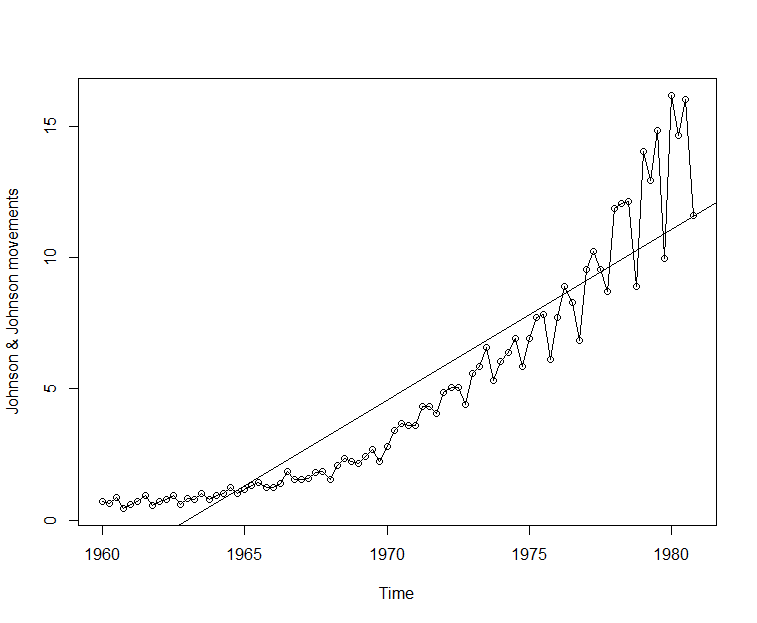
\includegraphics[width=0.7\linewidth]{../Beamer/linearreg}
\end{figure}
	
\end{frame}

\section{Preliminaries}
\subsection{White noise and Moving averages}
\begin{frame}{Preliminaries}{White noise and Moving averages}
\begin{itemize}
	\small{
\item In discrete time, white noise is a discrete signal whose samples are regarded as a sequence of serially \textit{uncorrelated random variables}, $ w_t $ , with mean $ 0 $ and variance $ \sigma^2 $. \\

\item Example: A single realization of white noise is a random shock. \\

\item A white noise process is one which has no correlation between its values at different times. \\ }
\end{itemize}

\pause	
\small {plot.ts(rnorm(200),col="blue",main="White noise") in R. }

\begin{figure}
\centering
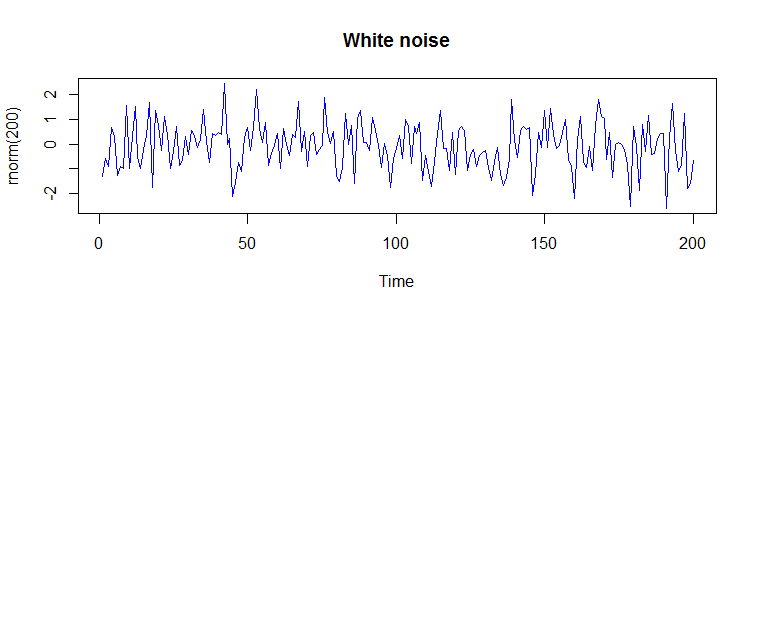
\includegraphics[width=0.8\linewidth]{whitenoise}
\caption{}
\end{figure}

\end{frame}

\begin{frame}{Preliminaries}{White noise and Moving averages}
The white noise $ w_t $ can be replaced by a moving average that \textit{smooths} the series. \\
Consider $ w_t $ as a average of its current value and its immediate neighbours. \\
\begin{equation}
v_t = \frac{1}{3} (w_{t-1}+w_t + w_{t+1})
\end{equation}



\end{frame}

\begin{frame}{Preliminaries}{White noise and Moving averages}
\small {Gaussian white noise series and three-point moving average of the Gaussian white noise series could like this. }

\begin{figure}
	\centering
	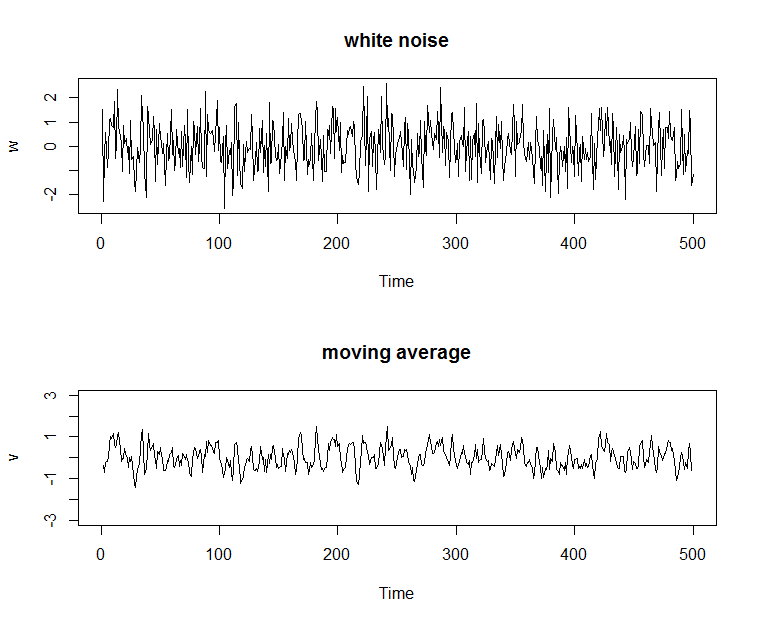
\includegraphics[width=0.75\linewidth]{Whitenoise_ma}
	\caption{Moving average smooth series}
	\label{}
\end{figure}

\end{frame}


\begin{frame}{Preliminaries}{White noise and Moving averages}
Equation (3) can be plotted in R using the \textit{filter} function in R. 

\begin{figure}
\centering
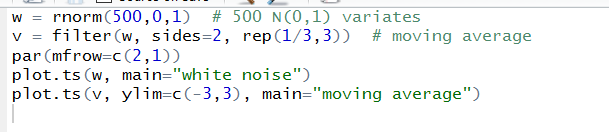
\includegraphics[width=\linewidth]{whitenoise_rcode}
\end{figure}


\end{frame}

\subsection{Stationary Series}
\begin{frame}{Preliminaries}{Stationary Series}

Modelling a time series (ARMA) model requires stationarity. 

% For an \textit{Auto Correlation function} (ACF) to make sense, the series must be a \textit{weakly stationary series}. This means that the autocorrelation for any particular lag is the same regardless of where we are in time.  

\pause
\begin{block}{Weak Stationary}
A series $ x_t $ is said to be (weakly) stationary if it satisfies the following properties:
\begin{itemize}
\item The mean $ E(x_t) $ is same for all $ t $
\item The variance  of $ (x_t) $ is same for all $ t $	
\item The covariance and the correlation between $ x_t $ and $ x_{t-h} $ is the same for all $ t $.
\end{itemize}
\end{block}
\end{frame}


\begin{frame}{Preliminaries}{Stationary Series} 	
\begin{figure}
\centering
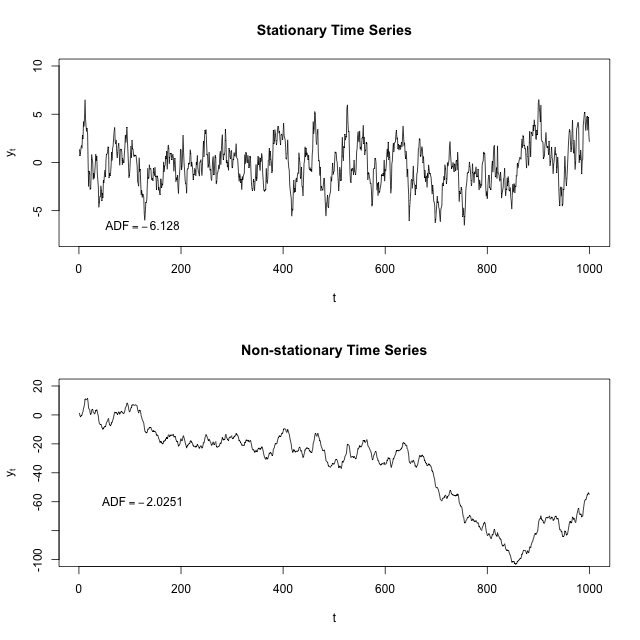
\includegraphics[width=0.6\linewidth]{Stationarycomparison}
\caption{Stationary vs Non stationary}
\label{}
\end{figure}
\end{frame}
		


\begin{frame}{Preliminaries}{Stationary Series}
Addressing non-stationary series. \pause
\begin{itemize}
\item Remove unequal variances. We do this using log of the series. 
\item We need to address the trend component. We do this by taking \textit{difference} of the series.
\item Differenced variable: $ \Delta x_t = x_t - x_{t-1}$
\end{itemize} 

This can be done using diff(log(JohnsonJohnson)) in R. 

\begin{figure}
\centering
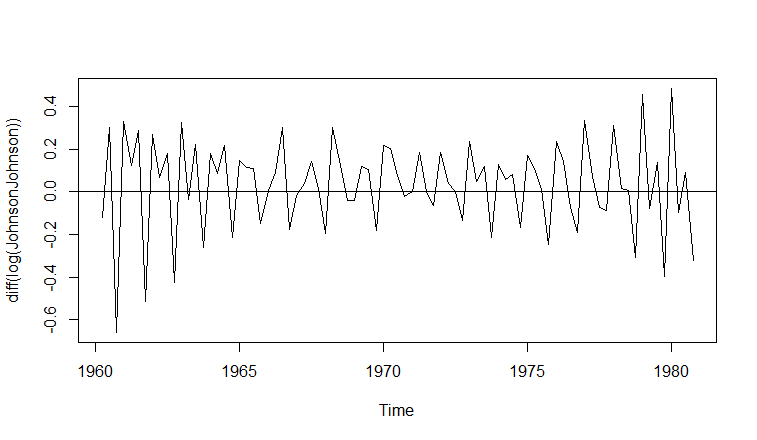
\includegraphics[width=0.6\linewidth]{difflog}
\end{figure}

\end{frame}


\begin{frame}{Preliminaries}{Augmented Dickey–Fuller test}
	\small{
Augmented Dickey–Fuller test \textbf{(ADF)} tests the null hypothesis of whether a unit root is present in a time series sample. The alternative hypothesis is usually stationarity or trend-stationarity. 

The testing procedure for the ADF test is applied to the AR(1) model;

\begin{equation}
x_t = \rho x_{t-1} + e_t
\end{equation}
}
\begin{align*}
x_t &: \text{is the variable of interest}\\
\rho &: \text{coefficient on a time trend} \\
e_t &: \text{error term}
\end{align*}


\small{A unit root is present if $ \rho=1 $. The model would be non-stationary in this case.}

\end{frame}

\begin{frame}{Preliminaries}{Augmented Dickey–Fuller test}
Estimation : We estimate if null-hypothesis is not rejected, then $ x_t $ is not stationary. \\
	
	
Testing ADF on our data JohnsonJohnson, in R, we have the following result. 

\begin{figure}
\centering
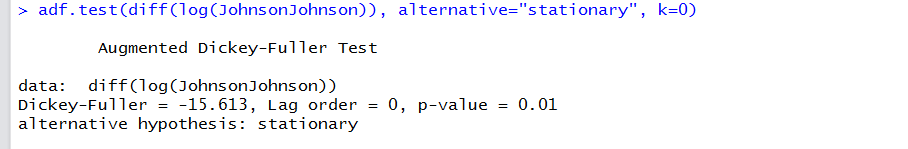
\includegraphics[width=1\linewidth]{ADFtest}
\end{figure}
	
\end{frame}	

\subsection{Autocorrelation function (ACF)}
\begin{frame}{Preliminaries}{Autocorrelation function (ACF)}
The ACF is a way to measure the linear relationship between an observation at time $ t $ and the observations at previous times. 	
	
	\begin{itemize}
\item $ x_t $ denote the value of a time series at time $ t $. \\
\item The ACF of the series gives correlations between $ x_t $ and $ x_{t-k} $ for $ k = 1, 2, 3, $ etc.  
\end{itemize}

Theoretically, the autocorrelation between $ x_t $ and $ x_{t-k} $ is, 	

\begin{equation*} 
ACF(k) = \frac{\text{Covariance}(x_t,  x_{t-k})}{\sigma_{{x_t}}. \sigma_{x_{t-k}}}  = \frac{\text{Covariance}(x_t, x_{t-k})}{\text{Variance}(x_t)}
\end{equation*}

\end{frame}

\begin{frame}{Preliminaries}{Autocorrelation function (ACF)}

\begin{figure}
	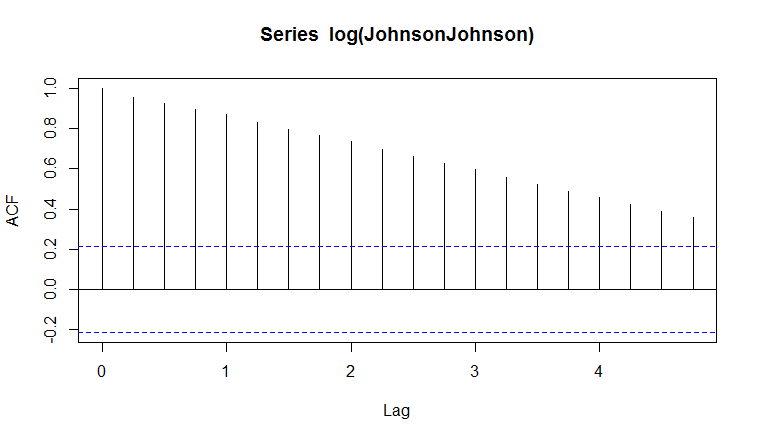
\includegraphics[width=0.475\textwidth]{ACF_log}
	\hfill
	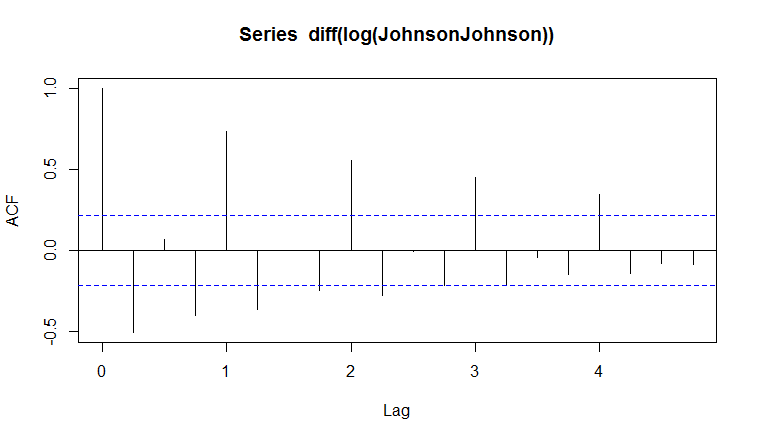
\includegraphics[width=0.475\textwidth]{ACF_logdiff}
	\caption{ACF of a non-stationary  vs stationary series}
\end{figure}
\small {The above ACF is “decaying”, or decreasing, very slowly, and remains well above the significance range (dotted blue lines). This is indicative of a non-stationary series.\\
	
On the other hand ACF of a stationary series shows exponential decay. This is indicative of a stationary series.}

\end{frame}

\subsection{Partial - Autocorrelation function (PACF)}
\begin{frame}{Preliminaries}{Partial - Autocorrelation function (PACF)}
PACF is a simple correlation between $ x_t $ and $ x_{t-k} $, minus the part explained by the intervening lags. 	

\begin{equation*}
\rho_k = Corr (x_t - E(x_t |x_{t-1} .... x_{t-k+1}),x_{t-k})
\end{equation*}

where; \\
$ E(x_t |x_{t-1} .... x_{t-k+1}) $ is the minimum squared error predictor. 

The 2nd order (lag) partial autocorrelation is; 

\begin{equation}
\frac{\text{Covariance}(x_t, x_{t-2}| x_{t-1})}{\sqrt{\text{Variance}(x_t|x_{t-1})\text{Variance}(x_{t-2}|x_{t-1})}}
\end{equation}
	
\end{frame}	

\begin{frame}{Preliminaries}{Partial - Autocorrelation function (PACF)}
PACF Plots	

\begin{figure}
\centering
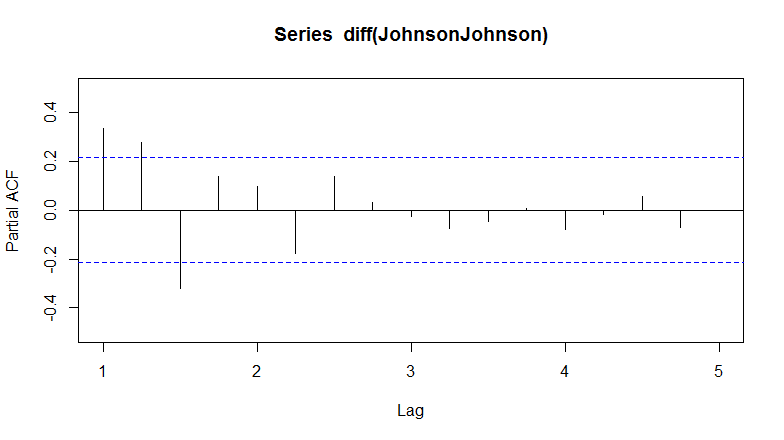
\includegraphics[width=0.8\linewidth]{pacf_jj}
\end{figure}

	
\end{frame}	

\section{First-order Autoregression Model (AR(1))}
\begin{frame}{First-order Autoregression Model (AR(1))} 	

AR(1) model is a linear model that predicts the present value of a time series using the immediately prior value in time.   In this model, the value of $ x $ at time $ t $ is a linear function of the value of $ x $ at time $ t–1 $.  Represented as; \\
\begin{equation*}  
x_{t}=\beta_{0}+\beta_{1}x_{t-1}+\epsilon_{t}  
\end{equation*}
	
\pause	
Assumptions:\\

$ \epsilon_t \overset{iid}{\sim} N(0, \sigma^2) $ i.e errors are independently distributed with a normal distribution that has mean 0 and constant variance.
	
An autoregressive model of order $ p $, AR(p), is of the form;  

\begin{equation}  
x_{t}=\beta_{0}+\beta_{1}x_{t-1}+\beta_{2}x_{t-2}+ .... \beta_{p}x_{t-p}+ \epsilon_{t}  
\end{equation}	
	
\end{frame}

\begin{frame}{First-order Autoregression Model (AR(1))} 

The mean of $ x_t $ is zero. If the mean $ \mu $ of $ x_t $ is not zero, we replace $ x_t $ by $ x_{t-\mu} $ in Equation(4) and write as; 	

\begin{equation}  
x_{t}=\alpha + \beta_{1}x_{t-1}+\beta_{2}x_{t-2}+ .... \beta_{p}x_{t-p}+ \epsilon_{t}  
\end{equation}

where $ \alpha = \mu(1-\beta_1.....- \beta_p) $. \\

We note that this equation is similar to the regression model of (1) and hence the term \textit{auto (or self) regression.}

\end{frame}	


\begin{frame}{First-order Autoregression Model (AR(1))}{Sample path of an AR(1) process}

\begin{figure}
\centering
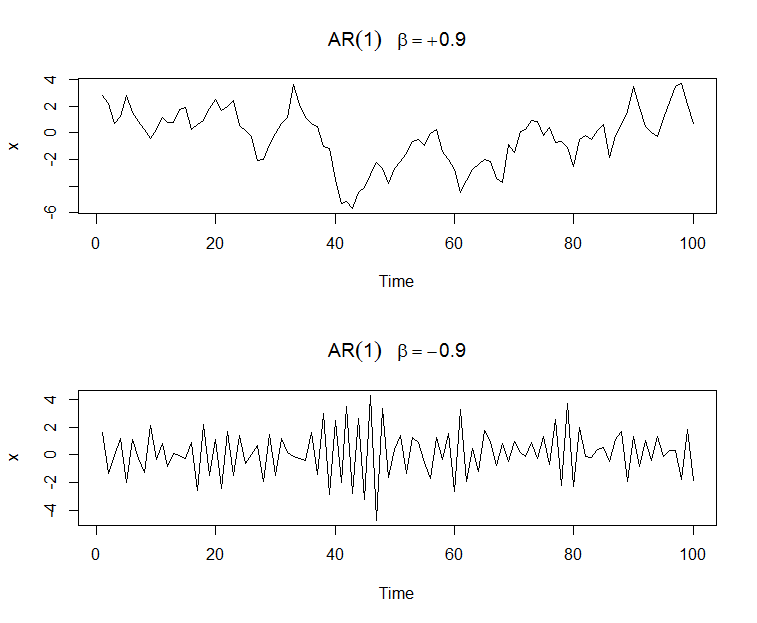
\includegraphics[width=0.8\linewidth]{AR(1)}
\end{figure}

\end{frame}

\begin{frame}{First-order Autoregression Model (AR(1))}{Sample path of an AR(1) process}
Plotted using the below R codes. 

\begin{figure}
\centering
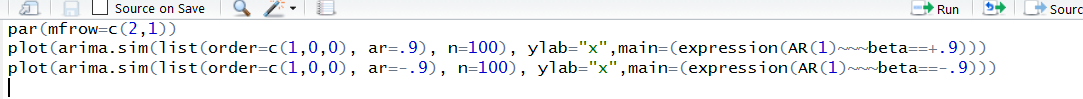
\includegraphics[width=\linewidth]{rcode2}
\end{figure}
	
\end{frame}	

\begin{frame}{First-order Autoregression Model (AR(1))}{ACF for AR(1)}
	
\begin{block}{}
	For an AR(1) model, the ACF is ACF(k) = $ \rho_k = \beta^k $. \\
	
	We say this function tails off. 
\end{block}	

\begin{figure}
\centering
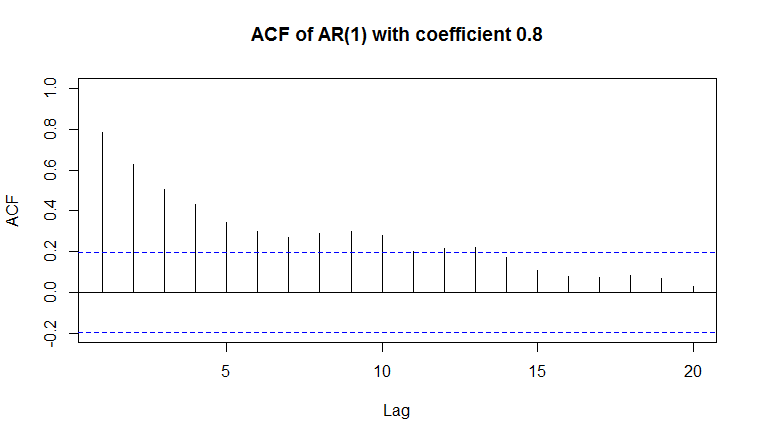
\includegraphics[width=0.9\linewidth]{ACF_ar1}
\end{figure}
\end{frame}

\begin{frame}{First-order Autoregression Model (AR(1))}{PACF for AR(1)}
\begin{figure}
\centering
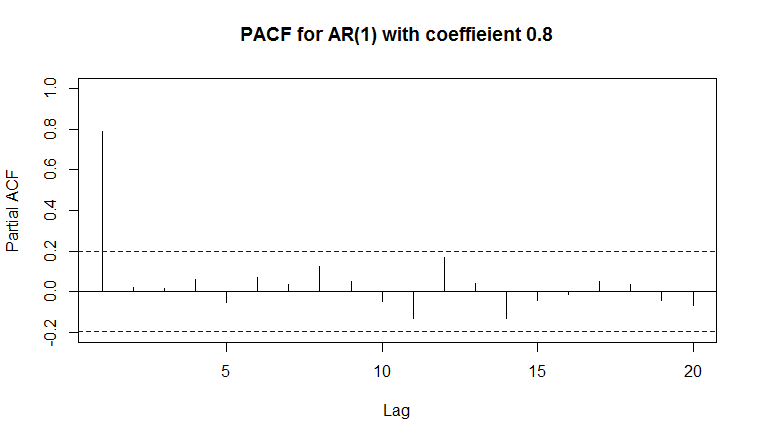
\includegraphics[width=0.9\linewidth]{ar1_pacf}
\end{figure}


\end{frame}

\section{Moving Average (MA) model}
\begin{frame}{Moving Average (MA) model}

The moving-average model specifies that the output variable depends linearly on the current and various past values.
	
A first order moving average model, denoted by MA(1) is	given by; 
\begin{equation*}
x_t =\mu + \epsilon_t +\theta_1\epsilon_{t-1}
\end{equation*}

and the \textit{qth} order moving average model with $ q $ lags, \textbf{MA(q)} is given by; 

\begin{equation*}
x_t = \epsilon_t +\theta_1\epsilon_{t-1}+\theta_2\epsilon_{t-2}+\dots + \theta_q\epsilon_{t-q}
\end{equation*}

where there are $ q $ lags in the moving average and $ \,\theta_1,\theta_2....\theta_q $ are parameters. 

\end{frame}



\begin{frame}{Moving Average (MA1) process}
\small{When for e.g $ \theta = 0.7 $,  $ x_t $ and $ x_{t-1} $ are positively correlated and when $ \theta = - 0.7 $, they are negatively correlated. }
\begin{figure}
\centering
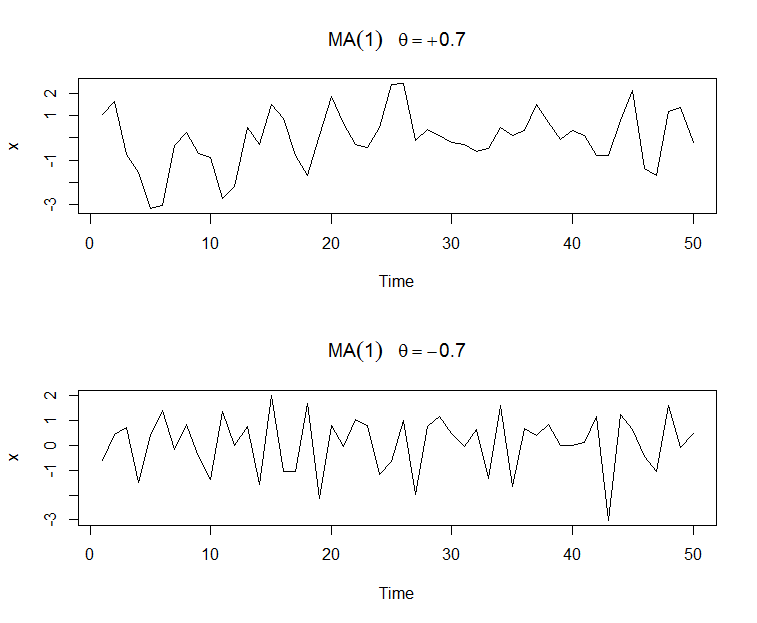
\includegraphics[width=0.65\linewidth]{ma1}
\end{figure}
\tiny{The above plot shows that the series is \textit{smoother} when $ \theta = 0.7 $. }

\end{frame}

\begin{frame}{Moving Average (MA1) process}
R code. 

\begin{figure}
\centering
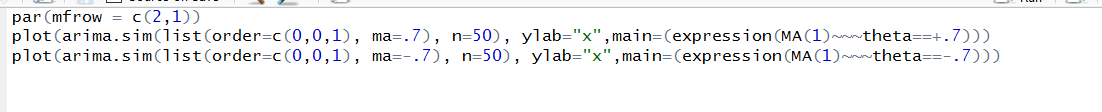
\includegraphics[width=\linewidth]{rcode3}
\end{figure}
	
	
\end{frame}

\section{ARMA model}
\begin{frame}{ARMA Model}
Autoregressive moving average (ARMA) models combine both $ p $ autoregressive terms and $ q $ moving average terms, also called ARMA(p,q) given by,

\begin{equation}
x_t = \beta_1 x_{t-1}+ .... +\beta_p x_{t-p} + \epsilon_t + \theta_1 \epsilon_{t-1} + ....  + \theta_q \epsilon_{t-q}
\end{equation}




\end{frame}

\section{Fitting the model (Summary)}
\begin{frame}{Fitting the model (Summary)}
Three items should be considered to determine a first guess at an ARIMA model: a time series plot of the data, the ACF, and the PACF.

\begin{itemize}
\item  Plot the data. Identify any unusual observations.
\item If the data are non-stationary: take first differences of the data until the data are stationary. 
\item For data with a curved upward trend accompanied by increasing variance, consider transforming the series with either a logarithm or a square root.
\item Examine the ACF/PACF: Is an AR(p) or MA(q) model appropriate?

\end{itemize}


\end{frame}
	
\begin{frame}[allowframebreaks]
\frametitle<presentation>{References}	
\begin{thebibliography}{10}
			
%\beamertemplatearticlebibitems			
%\bibitem{}

%\newblock {\em }

\beamertemplatebookbibitems			
\bibitem{}
Robert H. Shumway , David S. Stoffer
\newblock {\em Time Series analysis and its applications}


\beamertemplatebookbibitems			
\bibitem{}
Rob J Hyndman, George Athana­sopou­los
\newblock {\em Forecasting: Principles and practice}
			
\setbeamertemplate{bibliography item}[online]
\bibitem{}
The Pennsylvania State University - STAT 510 - Applied Time Series analysis
\newblock {\em }
\newblock \url{https://onlinecourses.science.psu.edu/stat510/}	
			
\setbeamertemplate{bibliography item}[online]
\bibitem{}
R Documentation
\newblock \url{https://www.rdocumentation.org/}	 						
			
\end{thebibliography}
\end{frame}

\begin{frame}
\centering
Thank You for your attention. 
\end{frame}


\end{document}